
%(BEGIN_QUESTION)
% Copyright 2006, Tony R. Kuphaldt, released under the Creative Commons Attribution License (v 1.0)
% This means you may do almost anything with this work of mine, so long as you give me proper credit

It is important for a thermocouple-based temperature instrument to have a {\it high input impedance}.  What does this mean, and why is it important in a thermocouple circuit?

\vskip 10pt

Modern digital voltmeter designs all exhibit high input impedance -- high enough for measuring thermocouple junction voltage, at least.  Suppose, though, you were asked to measure the output of a thermocouple {\it without} using any digital instruments.  You have plenty of analog voltmeter movements available, but they all have input impedances that are too low for this task.

Describe how you could build your own super-high input impedance voltmeter using readily available components.  Extra points for doing so without using an electronic circuit!

\underbar{file i00394}
%(END_QUESTION)





%(BEGIN_ANSWER)

When any electrical instrument is said to have a high input impedance, it means that it draws very little current from the source of voltage it is measuring.  This is true for any ideal voltmeter: that it measure voltage without ``loading'' the source of voltage by drawing substantial amounts of current from it.  It usually means that the instrument has a high DC resistance, but the word ``impedance'' implies other forms of opposition to electric current as well (namely capacitive and inductive reactance -- specific types of opposition to alternating current).

It is important for a thermocouple-based temperature instrument not to draw much current from the thermocouple it connects to, because thermocouple wires typically have greater electrical resistance per length than copper wires of similar gauge.  If there is substantial current in the thermocouple circuit, voltage will be dropped along the wire lengths, resulting in a measurement error:

$$\includegraphics[width=15.5cm]{i00394x04.eps}$$

\vskip 10pt

One way would be to build an operational amplifier (``op-amp'') buffer circuit to power an analog voltmeter movement.  Operational amplifiers typically have input impedances in the millions or billions of ohms (the TL082, an inexpensive, general-purpose JFET-input op-amp, has a typical input impedance of $10^{12} \> \Omega$ , or 1 {\it trillion} ohms!).  The circuit would look like this:

$$\includegraphics[width=15.5cm]{i00394x01.eps}$$

The op-amp senses the thermocouple's voltage signal and duplicates that voltage level at its output terminal, where it powers the meter movement.  The current necessary for powering the meter movement comes from the DC power supply (+V/-V) powering the op-amp, and not from the thermocouple, so the thermocouple circuit does not become ``loaded'' by the meter.  Another benefit of this strategy is that the op-amp buffer can easily be made into a precision amplifier, permitting the use of a larger-range voltmeter:

$$\includegraphics[width=15.5cm]{i00394x02.eps}$$

A non-electronic solution to this problem of building a high-impedance voltmeter is the classic ``null-balance'' or ``potentiometric'' voltmeter circuit, whereby an adjustable voltage source is used to balance the incoming signal voltage to be measured, with a highly sensitive ``null'' meter movement indicating when the two voltages are equal.  Then, a regular analog voltmeter reads how much voltage the adjustable voltage source is set for in this condition of balance:

$$\includegraphics[width=15.5cm]{i00394x03.eps}$$

In the balanced condition, the voltmeter movement's current requirements are supplied by the DC voltage source (battery), not the thermocouple.  In fact this type of circuit (null-balance, or ``potentiometric'') is the {\it only} type of voltage-measuring instrument hypothetically capable of attaining {\it infinite} input impedance.  Its simplicity and high theoretical input impedance makes it an elegant solution to the measurement problem.

%(END_ANSWER)





%(BEGIN_NOTES)


%INDEX% Measurement, temperature: thermocouple transmitter (high impedance input)

%(END_NOTES)


